\documentclass[floatsintext,man]{apa6}

\usepackage{amssymb,amsmath}
\usepackage{ifxetex,ifluatex}
\usepackage{fixltx2e} % provides \textsubscript
\ifnum 0\ifxetex 1\fi\ifluatex 1\fi=0 % if pdftex
  \usepackage[T1]{fontenc}
  \usepackage[utf8]{inputenc}
\else % if luatex or xelatex
  \ifxetex
    \usepackage{mathspec}
    \usepackage{xltxtra,xunicode}
  \else
    \usepackage{fontspec}
  \fi
  \defaultfontfeatures{Mapping=tex-text,Scale=MatchLowercase}
  \newcommand{\euro}{€}
\fi
% use upquote if available, for straight quotes in verbatim environments
\IfFileExists{upquote.sty}{\usepackage{upquote}}{}
% use microtype if available
\IfFileExists{microtype.sty}{\usepackage{microtype}}{}

% Table formatting
\usepackage{longtable, booktabs}
\usepackage{lscape}
% \usepackage[counterclockwise]{rotating}   % Landscape page setup for large tables
\usepackage{multirow}		% Table styling
\usepackage{tabularx}		% Control Column width
\usepackage[flushleft]{threeparttable}	% Allows for three part tables with a specified notes section
\usepackage{threeparttablex}            % Lets threeparttable work with longtable

% Create new environments so endfloat can handle them
% \newenvironment{ltable}
%   {\begin{landscape}\begin{center}\begin{threeparttable}}
%   {\end{threeparttable}\end{center}\end{landscape}}

\newenvironment{lltable}
  {\begin{landscape}\begin{center}\begin{ThreePartTable}}
  {\end{ThreePartTable}\end{center}\end{landscape}}




% The following enables adjusting longtable caption width to table width
% Solution found at http://golatex.de/longtable-mit-caption-so-breit-wie-die-tabelle-t15767.html
\makeatletter
\newcommand\LastLTentrywidth{1em}
\newlength\longtablewidth
\setlength{\longtablewidth}{1in}
\newcommand\getlongtablewidth{%
 \begingroup
  \ifcsname LT@\roman{LT@tables}\endcsname
  \global\longtablewidth=0pt
  \renewcommand\LT@entry[2]{\global\advance\longtablewidth by ##2\relax\gdef\LastLTentrywidth{##2}}%
  \@nameuse{LT@\roman{LT@tables}}%
  \fi
\endgroup}


  \usepackage{graphicx}
  \makeatletter
  \def\maxwidth{\ifdim\Gin@nat@width>\linewidth\linewidth\else\Gin@nat@width\fi}
  \def\maxheight{\ifdim\Gin@nat@height>\textheight\textheight\else\Gin@nat@height\fi}
  \makeatother
  % Scale images if necessary, so that they will not overflow the page
  % margins by default, and it is still possible to overwrite the defaults
  % using explicit options in \includegraphics[width, height, ...]{}
  \setkeys{Gin}{width=\maxwidth,height=\maxheight,keepaspectratio}
\ifxetex
  \usepackage[setpagesize=false, % page size defined by xetex
              unicode=false, % unicode breaks when used with xetex
              xetex]{hyperref}
\else
  \usepackage[unicode=true]{hyperref}
\fi
\hypersetup{breaklinks=true,
            pdfauthor={},
            pdftitle={Child language experience in a Tseltal Mayan village},
            colorlinks=true,
            citecolor=blue,
            urlcolor=blue,
            linkcolor=black,
            pdfborder={0 0 0}}
\urlstyle{same}  % don't use monospace font for urls

\setlength{\parindent}{0pt}
%\setlength{\parskip}{0pt plus 0pt minus 0pt}

\setlength{\emergencystretch}{3em}  % prevent overfull lines


% Manuscript styling
\captionsetup{font=singlespacing,justification=justified}
\usepackage{csquotes}
\usepackage{upgreek}

 % Line numbering
  \usepackage{lineno}
  \linenumbers


\usepackage{tikz} % Variable definition to generate author note

% fix for \tightlist problem in pandoc 1.14
\providecommand{\tightlist}{%
  \setlength{\itemsep}{0pt}\setlength{\parskip}{0pt}}

% Essential manuscript parts
  \title{Child language experience in a Tseltal Mayan village}

  \shorttitle{Child language experience in a Tseltal Mayan village}


  \author{Marisa Casillas\textsuperscript{1}, Penelope Brown\textsuperscript{1}, \& Stephen C. Levinson\textsuperscript{1}}

  % \def\affdep{{"", "", ""}}%
  % \def\affcity{{"", "", ""}}%

  \affiliation{
    \vspace{0.5cm}
          \textsuperscript{1} Max Planck Institute for Psycholinguistics  }

  \authornote{
    Correspondence concerning this article should be addressed to Marisa
    Casillas, P.O. Box 310, 6500 AH Nijmegen, The Netherlands. E-mail:
    \href{mailto:Marisa.Casillas@mpi.nl}{\nolinkurl{Marisa.Casillas@mpi.nl}}
  }


  \abstract{Enter abstract here. Each new line herein must be indented, like this
line.}
  \keywords{Child-directed speech, Linguistic input, Non-WEIRD, Vocal maturity, Turn
taking \\

    \indent Word count: X
  }





\usepackage{amsthm}
\newtheorem{theorem}{Theorem}[section]
\newtheorem{lemma}{Lemma}[section]
\theoremstyle{definition}
\newtheorem{definition}{Definition}[section]
\newtheorem{corollary}{Corollary}[section]
\newtheorem{proposition}{Proposition}[section]
\theoremstyle{definition}
\newtheorem{example}{Example}[section]
\theoremstyle{definition}
\newtheorem{exercise}{Exercise}[section]
\theoremstyle{remark}
\newtheorem*{remark}{Remark}
\newtheorem*{solution}{Solution}
\begin{document}

\maketitle

\setcounter{secnumdepth}{0}



\section{Introduction}\label{intro}

A great deal of work in developmental language science revolves around
one central question: What linguistic evidence (i.e., what types and how
much) is needed to support first language acquisition? In pursuing this
topic, many researchers have fixed their sights on the quantity and
characteristics of speech addressed to children; that is, speech
designed for young recipients who may have limited attention and
understanding. In several languages, child-directed speech
(CDS\footnote{Throughout this article, we use \enquote{child-directed
  speech} and \enquote{CDS} in the most literal sense: speech designed
  for and directed toward a child recipient.}) is linguistically
accommodated (Cristia, 2013; Soderstrom, 2007), interactionally rich
(Bruner, 1985; Butterworth, 2003; Estigarribia \& Clark, 2007; Masataka,
2003), and preferred by infants (Cooper \& Aslin, 1990; see, e.g., Hoff,
2006, and @golinkoff2015baby for reviews; preference, 2017; Segal \&
Newman, 2015). In those same linguistic communities, these properties of
CDS have been found to facilitate early word learning (Cartmill et al.,
2013; Hirsh-Pasek et al., 2015; e.g., Hoff, 2003; Hurtado, Marchman, \&
Fernald, 2008; M. L. Rowe, 2008; Laura A Shneidman \& Goldin-Meadow,
2012; Laura A Shneidman, Arroyo, Levine, \& Goldin-Meadow, 2012;
Weisleder \& Fernald, 2013). Yet ethnographic reports from a number of
traditional, non-Western communities suggest that children easily
acquire their community's language(s) even when they are infrequently
directly addressed (P. Brown, 2011). If so, CDS may not be essential for
learning language; just useful for facilitating certain aspects of
language development. In this paper we investigate the language
environment and early development of 10 Tseltal Mayan children growing
up in a community where caregivers are reported to infrequently directly
address speech to infants and young children (P. Brown, 8AD, 2011,
2014).

\subsection{Child-directed speech}\label{intro-cds}

Prior work on CDS in Western contexts has shown that the amount of CDS
children hear influences their language development; more CDS is
associated with larger and faster-growing receptive and productive
vocabularies in young children (e.g., Hart \& Risley, 1995; Hoff, 2003;
Hurtado et al., 2008; Ramírez-Esparza, García-Sierra, \& Kuhl, 2014,
2017; Laura A Shneidman \& Goldin-Meadow, 2012; Laura A Shneidman et
al., 2012; Weisleder \& Fernald, 2013; XX, XX). CDS has also been linked
to young children's speed of lexical retrieval (Hurtado et al., 2008;
Weisleder \& Fernald, 2013; but see XX, XX) and syntactic development
(Huttenlocher, Waterfall, Vasilyeva, Vevea, \& Hedges, 2010). The
conclusion drawn from much of this work is that speech directed to
children is well designed for learning words---especially concrete nouns
and verbs---because it is optimized for a child's attention and
understanding in the moment it is spoken. Even outside of first-person
interaction, infants and young children prefer listening to
attention-grabbing CDS over adult-directed speech (see preference, 2017
for a review). There are, however, a few significant caveats to the body
of work relating CDS quantity to language development.

First, while there is overwhelming evidence linking CDS quantity to
vocabulary size, links to grammatical development are more scant
(Brinchmann, Braeken, \& Lyster, 2019; Frank, Braginsky, Marchman, \&
Yurovsky, n.d.; e.g., Huttenlocher et al., 2010). While the advantage of
CDS for referential word learning is clear, it is less obvious how CDS
facilitates syntactic learning. For example, utterance length (a proxy
for syntactic complexity Wasow, 1997) doesn't appear to increase with
child age (Newport, Gleitman, \& Gleitman, 1977), and parents are less
likely to directly correct their children's syntactic errors than
semantic ones (R. Brown, 1977; but see Chouinard \& Clark, 2003)---even
sometimes themselves producing ungrammatical utterances to make
individual words salient to their young interlocutors (see also
{\textbf{???}}; R. N. Aslin, Woodward, LaMendola, \& Bever, 1996). On
the other hand, there is a wealth of evidence that syntactic knowledge
is lexically specified (Arnold, Wasow, Asudeh, \& Alrenga, 2004;
Goldberg, 2003; see, e.g., E. V. M. Lieven, Pine, \& Baldwin, 1997), and
that, crosslinguistically, children's vocabulary size is one of the most
robust predictors of their early syntactic development ({\textbf{???}};
Frank et al., n.d.; V. A. Marchman, Martínez-Sussmann, \& Dale, 2004).
In short, what is good for the lexicon may also be good for syntax. For
now, however, the link between CDS and other aspects of grammatical
development still needs to be more thoroughly tested.

A second caveat is that most work on CDS quantity uses summary measures
that average over the ebb and flow of interaction (e.g., proportion
CDS). In both child and adult interactions, verbal behaviors are highly
structured: while some occur at fairly regular intervals
(\enquote{periodic}, e.g., discourse connectives such as
\enquote{alright}, \enquote{okay}, and \enquote{well}), others occur in
shorter, more intense bouts separated by long periods of inactivity
(\enquote{bursty}, e.g., content words, descriptions; Abney, Dale,
Louwerse, and Kello (2018), see also Fusaroli, Razczaszek-Leonardi, and
Tylén (2014)). For example, Abney and colleagues (2017) found that,
across multiple time scales of daylong recordings, both infants' and
adults' vocal behavior was clustered. Focusing on lexical development,
Blasi and colleagues (in preparation) also found that nouns and verbs
were used burstily in child-proximal speech across all six of the
languages in their typologically diverse sample. Infrequent words were
somewhat more bursty overall, leading them to propose that burstiness
may play a key and universal role in acquiring otherwise-rare linguistic
units. Experiment-based work also shows that two-year-olds learn novel
words better from a massed presentation of object labels versus a
distributed presentation (but see Ambridge, Theakston, Lieven, \&
Tomasello, 2006, and @childers2002two; Schwab \& Lew-Williams, 2016).
Structured temporal characteristics in children's language experience
imply new roles for attention and memory in language development. By
that token, we should begin to investigate the link between CDS and
linguistic development with more nuanced measures of how CDS is
distributed.

Finally, prior work has typically focused on Western (primarily North
American) populations, limiting our ability to generalize these effects
to children acquiring language worldwide (P. Brown \& Gaskins, 2014;
Henrich, Heine, \& Norenzayan, 2010; E. V. M. Lieven, 1994; M. Nielsen,
Haun, Kärtner, \& Legare, 2017). While we do gain valuable insight by
looking at \emph{within-population} variation (e.g., different
socioeconomic or sub-cultures), we can more effectively find places
where our assumptions break down by studying \emph{new} populations.
Linguistic anthropologists working in non-Western communities have long
reported that caregiver interaction styles vary immensely from place to
place, with some caregivers using little or no CDS to young children (P.
Brown \& Gaskins, 2014; Gaskins, 2006; E. V. M. Lieven, 1994). Children
in these communities reportedly acquire language with
\enquote{typical}-looking benchmarks. For example, they start pointing
and talking around the same time we would expect for Western
middle-class infants (e.g., P. Brown, 2011, 2014; P. Brown \& Gaskins,
2014; Liszkowski, Brown, Callaghan, Takada, \& De Vos, 2012; but see
also Salomo \& Liszkowski, 2013). These findings have had little impact
on mainstream theories of word learning and language acquisition, partly
due to a lack of directly comparable measures (P. Brown, 2014; P. Brown
\& Gaskins, 2014). If, however, these children indeed acquire language
without delay despite little or no CDS, we must reconsider what kind of
linguistic evidence is necessary for children to learn language.

\subsection{Language development in non-WEIRD
communities}\label{intro-nonweird}

A growing number of researchers are using methods from developmental
psycholinguistics to describe the language environments and linguistic
development of children growing up in traditional and/or non-Western
communities (Barrett et al., 2013; see also, e.g., Demuth, Moloi, \&
Machobane, 2010; Fortier, Kellier, Fernández Flecha, \& Frank, under
review; Ganek, Smyth, Nixon, \& Eriks-Brophy, 2018; Garcia, Roeser, \&
Höhle, 2018; Hernik \& Broesch, 2018). We briefly highlight two recent
efforts along these lines, but see Cristia and colleagues (2017) and
Mastin and Vogt's work (2016; 2015) for similar examples.

Scaff, Cristia, and colleagues (2017; In preparation) have used a number
of methods to estimate how much speech children hear in a Tsimane
forager-horticulturalist population in the Bolivian lowlands. From
daylong audio recordings, they estimate that Tsimane children between
0;6 and 6;0 hear maximally \textasciitilde{}5 minutes of directly
addressed speech per hour, regardless of their age (but see Cristia et
al., 2017). For comparison, children from North American homes between
ages 0;3 and 3;0 are estimated to hear \textasciitilde{}11 minutes of
CDS per hour in daylong recordings (Bergelson et al., 2018b). Tsimane
children also hear \textasciitilde{}10 minutes of other-directed speech
per hour (e.g., talk between adults) compared to the \textasciitilde{}7
minutes per hour heard by young North American children (Bergelson et
al., 2018b). This difference may be attributable to the fact that the
Tsimane live in extended family clusters of 3--4 households, so speakers
are typically in close proximity to 5--8 other people (Cristia et al.,
2017).

Shneidman and colleagues (2010; 2012) analyzed speech from one-hour
at-home video recordings of children between ages 1;0 and 3;0 in two
communities: Yucatec Mayan (Southern Mexico) and North American (a major
U.S. city). Their analyses yielded four main findings: compared to the
American children, (a) the Yucatec children heard many fewer utterances
per hour, (b) a much smaller proportion of the utterances they heard
were \emph{child-directed}, (c) the proportion of utterances that were
child-directed increased dramatically with age, matching U.S. children's
by 3;0 months, and (d) most of the added CDS came from other children
(e.g., older siblings and cousins). They also demonstrated that the
lexical diversity of the CDS they hear at 24 months---particularly from
adult speakers---predicted children's vocabulary knowledge at 35 months.

These groundbreaking studies establish a number of important findings:
First, children in each of these communities appear able to acquire
their languages with relatively little CDS. Second, CDS might become
more frequent as children get older, though this could largely be due to
speech from other children. Finally, despite these differences, CDS from
adults may still be the most robust predictor of vocabulary growth.

\subsection{The current study}\label{intro-currentstudy}

We examine the early language experience of 10 Tseltal Mayan children
under age 3;0. Prior ethnographic work suggests that Tseltal caregivers
do not frequently speak directly to their children until the children
themselves begin to actively initiate verbal interactions (P. Brown,
2011, 2014). Nonetheless, Tseltal children develop language with no
apparent delays. Tseltal Mayan language and culture has much in common
with the Yucatec Mayan communities Shneidman reports on, allowing us to
compare differences in child language environments between the two sites
more directly than before.\footnote{For a review of comparative work on
  language socialization in Mayan cultures, see Pye (2017).} We provide
more details on this community and dataset in the
\protect\hyperlink{methods}{Methods section}.

Similar to previous work, we estimated how much other-directed speech
children could have listened to, how much was directed to them, and how
those quantities changed with age. To this foundation we added new
sampling techniques for investigating variability in children's speech
environments within daylong recordings. We also analyzed children's
early vocal productions, examining both the overall developmental
trajectory of their vocal maturity and how their vocalizations are
influenced by CDS.

Based on prior work, we predicted that Tseltal Mayan children hear
little CDS, that the amount of CDS they hear increases with age, that
most CDS comes from other children, and that, despite this, Tseltal
Mayan children reach speech production benchmarks on par with Western
children. We additionally predicted that children's language
environments would be bursty---that brief, high-intensity interactions
would be sparsely distributed throughout the day, accounting for the
majority of children's daily CDS. \textbf{{[}TASK: REVISIT THIS{]}}

\hypertarget{methods}{\section{Methods}\label{methods}}

\subsection{Community}\label{methods-community}

The children in our dataset come from a small-scale, subsistence farming
community in the highlands of Chiapas in Southern Mexico. The vast
majority of children grow up speaking Tseltal monolingually at home. The
first few years of primary school are conducted mainly in Tseltal, but
the remainder of primary school, secondary school, and any further
education is conducted exclusively in Spanish. Nuclear families are
often large (5+ children) and live in patrilineal clusters. Nearly all
families grow staple crops such as corn and beans, but also bananas,
chilies, squash, coffee, and more. Household and farming work is divided
among men, women, and older children. Women do much of the daily
cleaning and food preparation, but also frequently work in the garden,
haul water and firewood, and do other physical labor. A few community
members---both men and women---earn incomes as teachers and shopkeepers
but are still expected to regularly contribute to their family's
household work.

More than forty years of ethnographic work by the second author has
reported that Tseltal children's language environments are
non-child-centered and non-object-centered (P. Brown, 8AD, 2011, 2014).
During their waking hours, Tseltal infants are typically tied to their
mother's back while she goes about her work for the day. Infants receive
very little direct speech until they themselves begin to initiate
interactions, usually as they approach their first birthdays. Even then,
interactional exchanges are often brief or non-verbal (e.g., object
exchange routines) and take place within a multi-participant context (P.
Brown, 2014). Rarely is attention given to words and their meanings,
even when objects are central to the activity. Instead, interactions
tend to focus on appropriate actions and responses, and young children
are socialized to attend to the interactions taking place around them
(León, 2011; see also Rogoff, Paradise, Arauz, Correa-Chávez, \&
Angelillo, 2003).

Young children are often cared for by other family members, especially
older siblings. Even when not on their mother's back, infants are rarely
put on the ground, so they can't usually pick up the objects around them
until they are old enough to walk. Toys are scarce and books are
vanishingly rare, so the objects children do get their hands on tend to
be natural or household objects (e.g., rocks, sticks, spoons, baskets,
etc.). By age five, most children are competent speakers who engage
daily in chores and caregiving of their younger siblings. The Tseltal
approach to caregiving is similar to that described for other Mayan
communities (Gaskins, 1996, 1999; León, 1998, 2011; e.g., Pye, 1986;
Rogoff et al., 1993, 2003; Laura A Shneidman \& Goldin-Meadow, 2012).

\subsection{Corpus}\label{methods-corpus}

The current data come from the Casillas HomeBank Corpus (Casillas,
Brown, \& Levinson, 2017; VanDam et al., 2016), which includes daylong
recordings and other developmental language data from more than 100
children under 4;0 across two indigenous, non-WEIRD communities: the
Tseltal Mayan community described here and a Papua New Guinean community
described elsewhere (P. Brown, 2011, 2014; P. Brown \& Casillas, in
press).

\emph{{[}TASK: Check these demographic data again{]}} The Tseltal data,
primarily collected in 2015, include recordings from 55 children born to
43 mothers. The families in our dataset typically only had 2--3 children
(median = 2; range = 1--9), due to the fact that the participating
families come from a young subsample of the community (mothers: mean =
26.9 years; median = 25.9; range = 16.6--43.8 and fathers: mean = 30.5;
median = 27.6; range = 17.7---52.9). On average, mothers were 20.1 years
old when they had their first child (median = 19; range = 12--27), with
a following inter-child interval of 3.04 years (median = 2.8; range =
1--8.5).\footnote{These estimates do not include miscarriages and/or children who passed away.}.
As a result, 26\% of the participating families had two children under
4;0. To our knowledge at time of recording, all children were typically
developing. We calculated the precise age of children based on the
birthdates given by their caregivers, though these should be taken with
a pinch of salt because documentation and reporting of birthdates is
less rigorous than is typically expected for studies based on Western
post-industrial populations.

Households size, defined in our dataset by the number of people sharing
a kitchen or other primary living space, ranged between between 3 and 15
people (mean = NN; median = NN). Although 30.9\% of the target children
are first-born, they were rarely the only child in their household.
Caregiver education is one (imperfect) measure of contact with Western
culture. Most mothers had finished primary school, with many also having
completed secondary school (range = no schooling--university). Most
fathers had finished secondary school, with many having also completed
preparatory school (range = no schooling--university). Clan membership
influences marriage and land inheritance such that 93\% of the fathers
grew up in the village where the recordings took place, while only 53\%
of the mothers did.

\subsubsection{Recordings}\label{methods-corpus-recs}

Methods for estimating the quantity of speech that children hear have
advanced significantly in the past two decades, with long-format at-home
audio recordings quickly becoming the new standard (e.g., with the
LENA\textsuperscript{®} system; Greenwood, Thiemann-Bourque, Walker,
Buzhardt, \& Gilkerson, 2011). These recordings capture a wider range of
the linguistic patterns children hear as they participate in different
activities with different speakers over the course of their day. In
long-format recordings, caregivers also tend to use less CDS (see also
Bergelson, Amatuni, Dailey, Koorathota, \& Tor, 2018a; C. Tamis-LeMonda,
Kuchirko, Luo, Escobar, \& Bornstein, 2017)\footnote{Typically, the
  CDS-features measured in these studies correlated between short- and
  long-format recordings, but with some caveats.}. The goal of these
recordings is to more or less capture a representative sample of what
the child hears and says at home.

\begin{figure}

{\centering 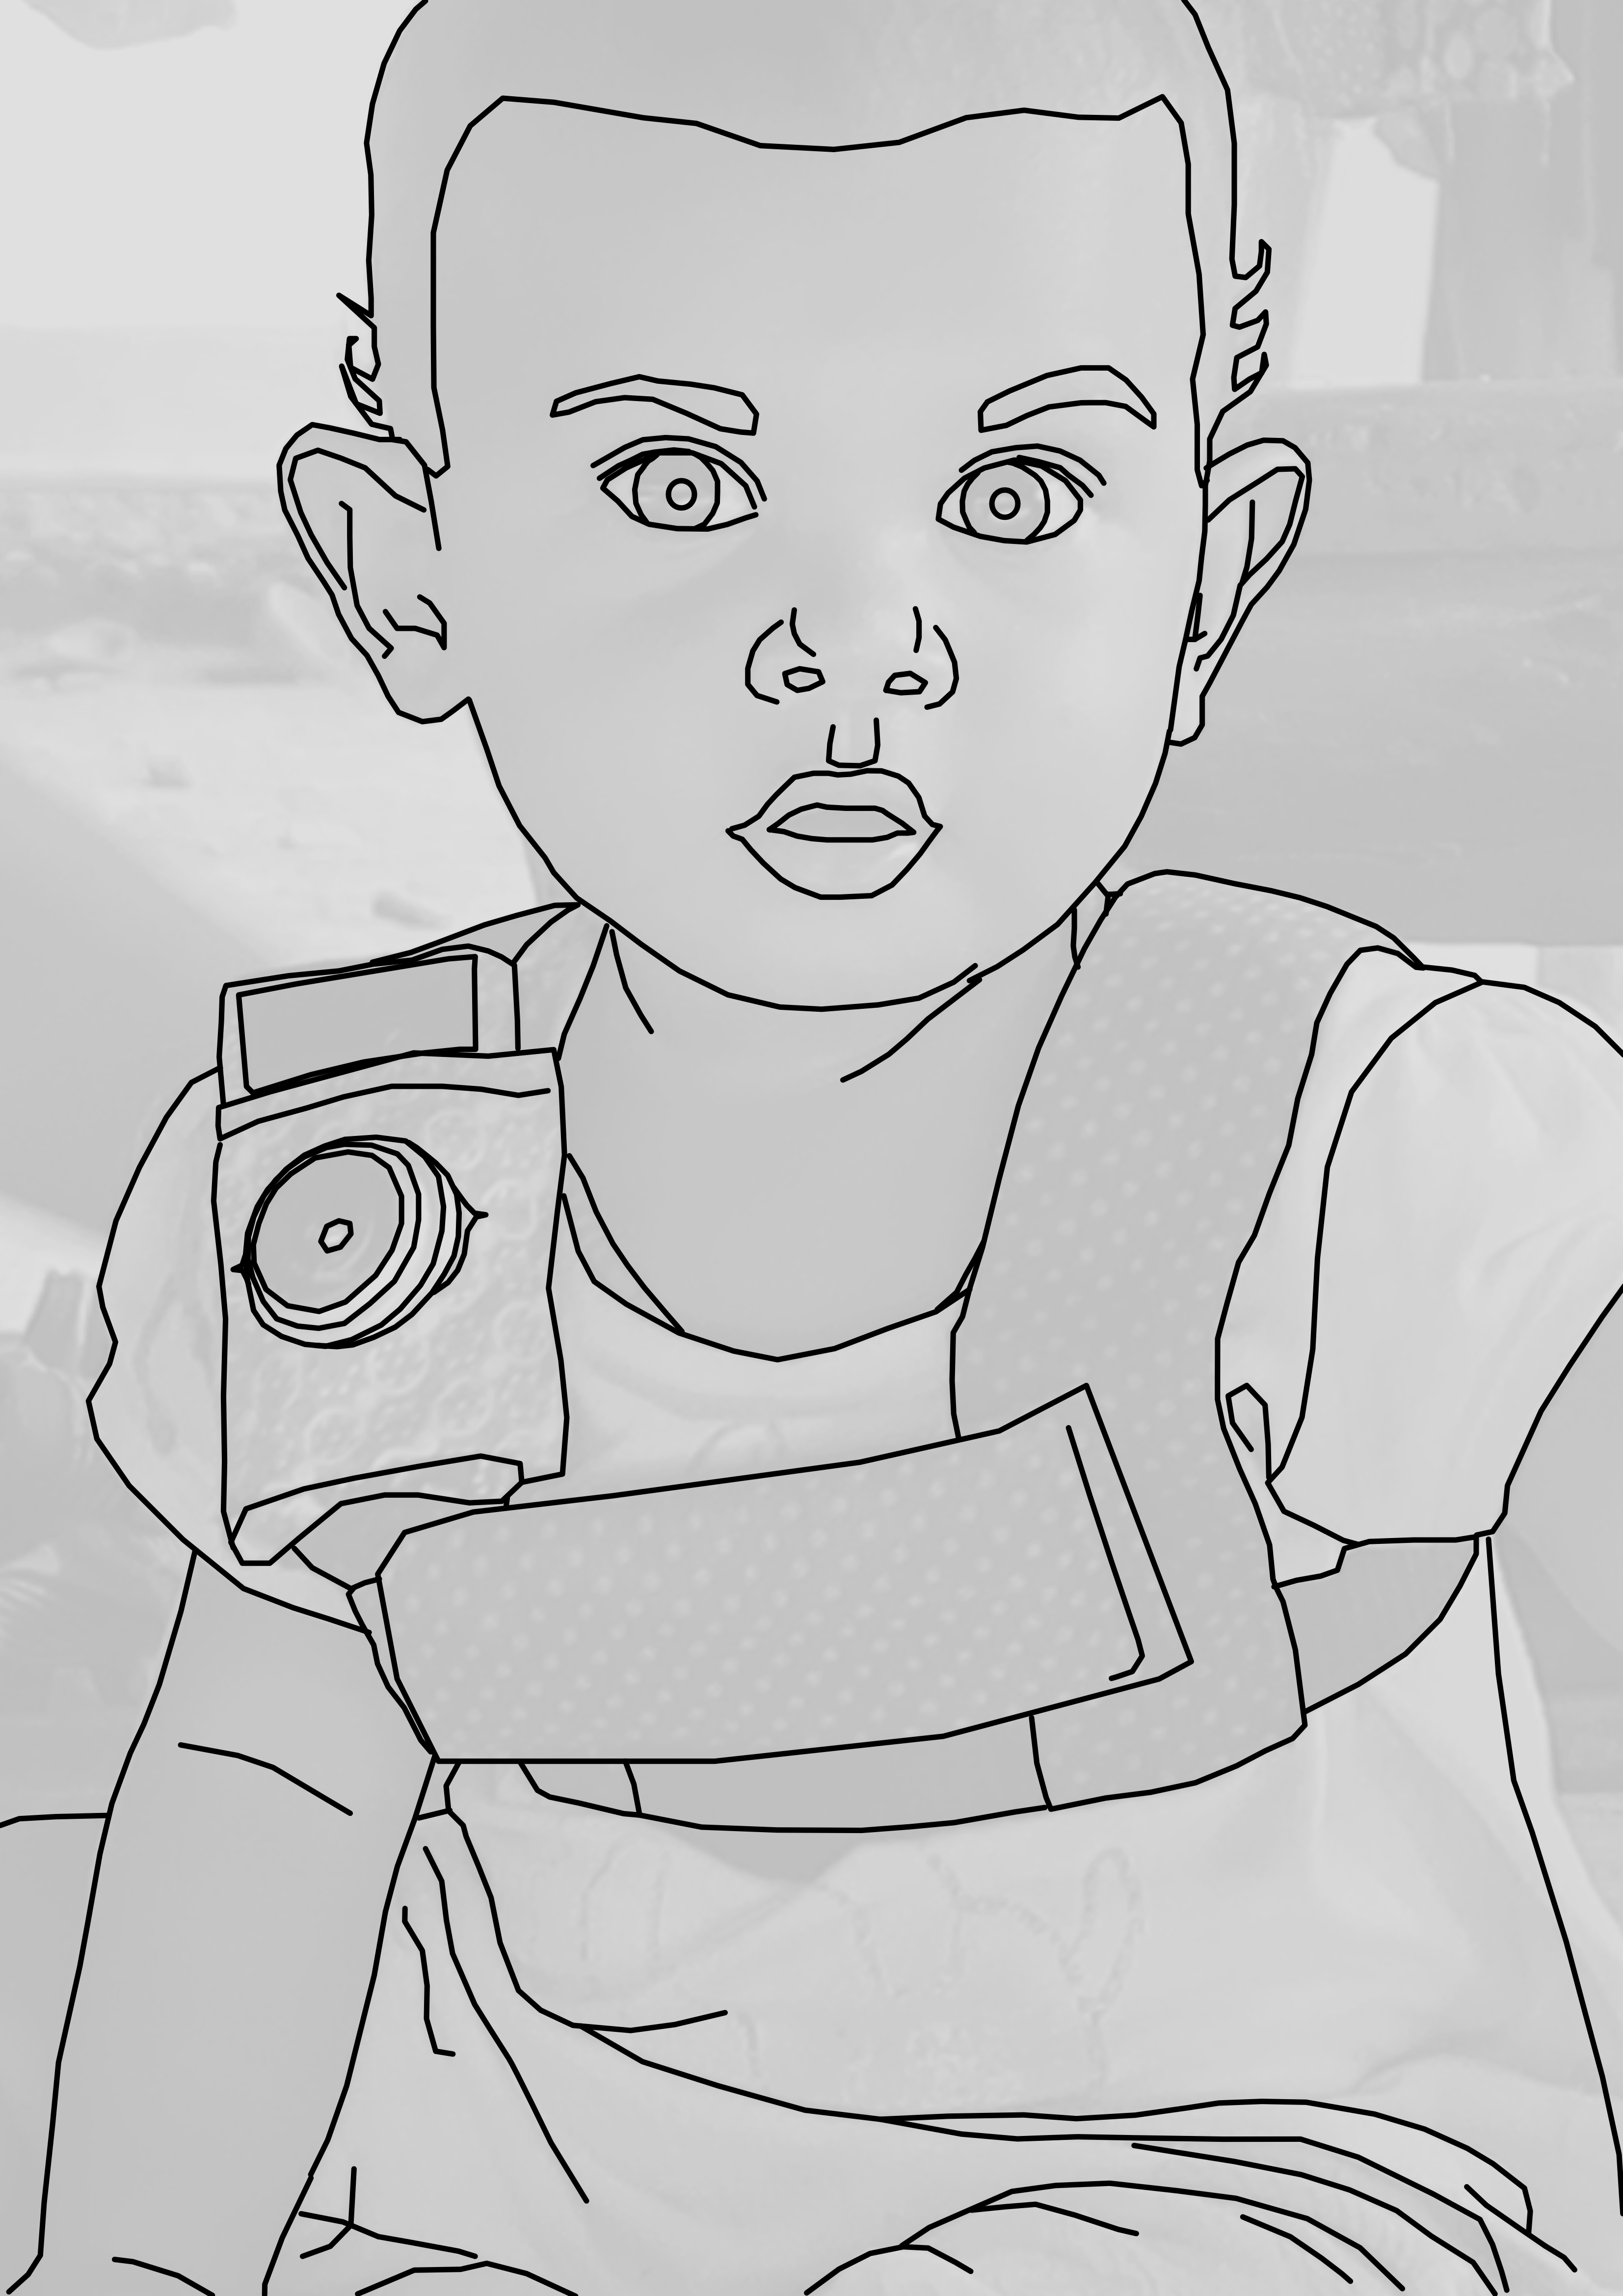
\includegraphics[width=0.5\linewidth]{Tseltal-CLE_files/TseltalCLE-RecordingVest} 

}

\caption{The recording vest fit over children's chests with an audio recording device in the front horizontal pocket and a camera fitted with a fisheye lens attached to the a shoulder strap.}\label{fig:fig1}
\end{figure}

We used a novel combination of a lightweight stereo audio recorder
(Olympus\textsuperscript{®} WS-832) and wearable photo camera (Narrative
Clip 1\textsuperscript{®}) fitted with a fish-eye lens, to track
children's movements and interactions over the course of a 9--11-hour
period in which the experimenter was not present. Each recording was
made during a single day at home in which the recorder and/or camera was
attached to the child. Ambulatory children wore both devices on an
elastic vest. Non-ambulatory children wore the recorder in a onesie
while their primary caregiver wore the camera on an elastic vest (see
\protect\hyperlink{fig1}{Figure 1}). The camera was set to take photos
at 30-second intervals and was synchronized to the audio in
post-processing to create a video file featuring the snapshot-linked
audio from the child's recording.\footnote{Documentation and scripts for
  post-processing are available at and
  \url{https://github.com/marisacasillas/Weave}.}

\subsection{Data selection and annotation}\label{methods-samples}

We annotated video clips from 10 of the 55 children's recordings. We
chose these 10 recordings to maximize variance in three demographic
variables: child age (0--3;0), child sex, and maternal education. The
sample is summarized in \emph{Table 1} \emph{{[}TASK: Make table{]}}. We
then selected one hour's worth of non-overlapping clips from each
recording in the following order: nine randomly selected 5-minute clips,
five 1-minute clips manually selected as the top \enquote{turn-taking}
minutes of the recording, five 1-minute clips manually selected as the
top \enquote{vocal activity} minutes of the recording, and one, manually
selected 5-minute extension of the best 1-minute sample (see
\protect\hyperlink{fig2}{Figure 2}). We created these different
subsamples of each day to measure properties of (a) children's
\emph{average} language environments (random samples) and (b) their
\emph{most input-dense} language environments (turn-taking samples). The
third sample (high-activity) gave us insight into children's productive
speech abilities.

The turn-taking and high-activity clips were chosen by two trained
annotators (the first author and a student assistant) who listened to
each recording in its entirety at 1--2x speed while actively taking
notes about potentially useful clips. Afterwards, the first author
reviewed the list of candidate clips, listened again to each one (at 1x
speed, multiple repetitions), and chose the best five 1-minute samples
for each of the two types of activity. Good turn-taking activity was
defined as closely timed sequences of contingent vocalization between
the target child and at least one other person (i.e., frequent
vocalization exchanges). The \enquote{best} turn-taking clips were
chosen because they had the most and most clear turn-switching activity
between the target child and the other speaker(s). Good vocal activity
clips were defined as clips in which the target child produced the most
and most diverse spontaneous (i.e., not imitative) vocalizations. The
\enquote{best} vocal activity clips were chosen for representing the
most linguistically mature and/or diverse vocalizations made by the
child over the day. All else being equal, candidate clips were
prioritized when they contained less background noise or featured
speakers and speech that were not otherwise frequently represented
(e.g., CDS from older males). The best turn-taking clips and vocal
activity clips often overlapped; turn-taking clips were selected from
the list of candidates first, and then vocal-activity clips were chosen
from the remainder. The instructions for selecting clips and resulting
notes can be found at
\url{https://github.com/marisacasillas/Tseltal-CLE/blob/master/audio_scanning_instructions.md}.

\begin{figure}
\centering
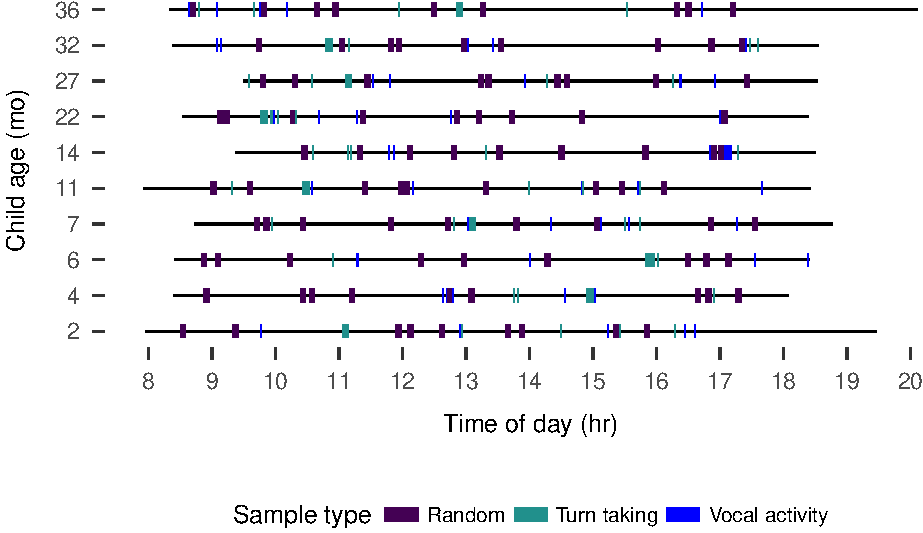
\includegraphics{Tseltal-CLE_files/figure-latex/fig2-1.pdf}
\caption{\label{fig:fig2}Recording duration (black line) and sampled clips
(colored boxes) for each recording analyzed, sorted by child age.}
\end{figure}

Each video clip was transcribed and annotated in ELAN (Wittenburg,
Brugman, Russel, Klassmann, \& Sloetjes, 2006) using the ACLEW
Annotation Scheme (Casillas et al., 2017) by the first author and a
native speaker of Tseltal who lives in the community and knows most of
the recorded families personally. The annotations include the
transcription of (nearly) all hearable utterances in Tseltal, a loose
translation of each utterance into Spanish, vocal maturity measures of
each target child utterance (non-linguistic vocalizations/non-canonical
babbling/non-word canonical babbling/single words/multiple words), and
addressee annotations for all non-target-child utterances
(target-child-directed/other-child-directed/adult-directed/adult-and-child-directed/animal-directed/other-speaker-type-directed).
We annotated each utterance for intended addressee using contextual
interactional information from the photos, audio, and
preceding/following footage; we used an \enquote{unsure} category for
utterances without sufficient evidence for confident
classification.\footnote{Full documentation, including training
  materials, for the ACLEW Annotation Scheme can be found at
  \url{https://osf.io/b2jep/wiki/home/}.} We exported each ELAN file as
tab-separated values for analysis.

\subsection{Data analysis}\label{methods-analysisinfo}

In what follows, we first describe quantitative characteristics of
children's speech environments, as captured by the 9 randomly selected
five-minute clips for each child. We report five measures:
target-child-directed speech (TCDS) and other-directed speech (ODS)
minutes per hour, the number of target-child-to-other (TC--O) and
other-to-target-child (O-TC) turn transitions per minute, and the
duration of the target child's interactional sequences in seconds. We
then briefly review these same speech environment characteristics for
the 5--6 one- or five-minute turn-taking clips\footnote{The turn-taking
  clips included in this analysis are: the 5 one-minute turn-taking
  clips and also the five-minute \enquote{extension} clip for that
  recording if it was an extension of a turn-taking clip.}, as
representative \enquote{peak} interactional moments in the day and
investigate how many minutes in the day are likely to have these
characteristics.

\section{Results}\label{results}

\emph{{[}TASK: change fits in the figures to reflect model estimates{]}}

\subsection{Data analysis}\label{data-analysis}

Unless otherwise stated, all analyses were conducted with generalized
linear mixed-effects regressions using the glmmTMB package and all plots
are generate with ggplot2 in R (Brooks et al., 2017a; R Core Team, 2018;
Wickham, 2009).\footnote{The data and analysis code are freely available
  on the web ({[}retracted for review{]}), as is a summary of the
  results which will be updated as more transcriptions become available
  ({[}retracted for review{]}).} Notably, all five speech environment
measures are restricted to non-negative values (min/hr, turn
transitions/min, and duration in seconds), with a subset of them also
displaying extra cases of zero in the randomly sampled clips (min/hr,
turn transitions/min; e.g., when the child is napping). The consequence
of these boundary restrictions is that the variance of the distributions
becomes non-gaussian (i.e., a long right tail). We account for this
issue by using negative binomial regression, whish is useful for
overdispersed count data (Brooks et al., 2017b; Smithson \& Merkle,
2013). When extra cases of zero are present due to, e.g., no speakers
being present, we used a zero-inflation negative binomial regression,
which creates two models: (a) a binary model to evaluate the likelihood
of none vs.~some presence of the variable (e.g., TCDS) and (b) a count
model of the variable (e.g., \enquote{3} vs. \enquote{5} TCDS min/hr),
using the negative binomial distribution as the linking function.
Alternative analyses using gaussian models with logged dependent
variables are available in the Supplementary Materials, but are
qualitatively similar to the results we report here.

Our primary predictors were as follows: child age (months), household
size (number of people), and number of non-target-child speakers present
in that clip, all centered and standardized, plus squared time of day at
the start of the clip (in decimal hours; centered on noon and
standardized). We always used squared time of day to model the cycle of
activity at home: the mornings and evenings should be more similar to
each other than midday because people tend to disperse for chores after
breakfast. To this we also added two-way interactions between child age
and number of speakers present, household size, and time of day.
Finally, we included a random effect of child, with random slopes of
time of day, unless doing so resulted in model non-convergence. Finally,
for the zero-inflation models, we included child age, number of speakers
present, and time of day. We have noted below when models needed to
deviate from this core design to achieve convergence. We only report
significant effects here; full model outputs are available in the
Supplementary Materials.

\begin{figure}
\centering
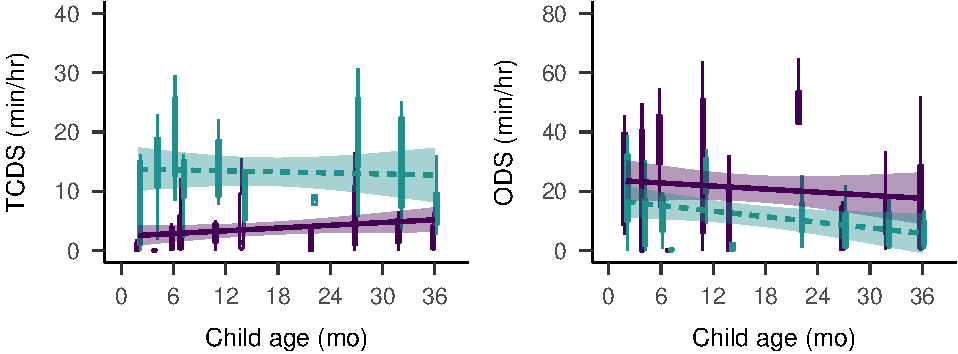
\includegraphics{Tseltal-CLE_files/figure-latex/fig3-1.pdf}
\caption{\label{fig:fig3}By-child estimates of minutes per hour of
other-directed speech (left) and target-child-directed speech (right).
Data are shown for the random (purple; solid) and turn taking (green;
dashed) samples. Bands on the solid linear trends show 95\% CIs.}
\end{figure}

\subsection{Target-child-directed speech
(TCDS)}\label{target-child-directed-speech-tcds}

The Tseltal children in our study were directly spoken to for an average
of 3.63 minutes per hour in the random sample (median = 4.08; range =
0.83--6.55; \protect\hyperlink{fig3}{Figure 3}). These estimates are
close to those reported for Yucatec Mayan data (Laura A Shneidman \&
Goldin-Meadow, 2012), which are plotted with our data, along with
estimates from a few other populations in
\protect\hyperlink{fig4}{Figure 4} (US/Canada: Bergelson et al., 2018b;
Tsimane: Scaff et al., In preparation, see {\textbf{???}} for a more
detailed comparison; US urban and Yukatek: Laura A. Shneidman, 2010;
Mozambique urban and rural, and Dutch: Vogt et al., 2015).\footnote{We
  convert the original estimates from Laura A. Shneidman (2010) into
  min/hr by using the median utterance duration in our dataset for all
  non-target child speakers: (1029ms). Note that, though this conversion
  is far from perfect, Yukatek and Tseltal are related languages.}. We
modeled TCDS min/hr in the random clips with a zero-inflated negative
binomial regression, as described above.

\begin{figure}
\centering
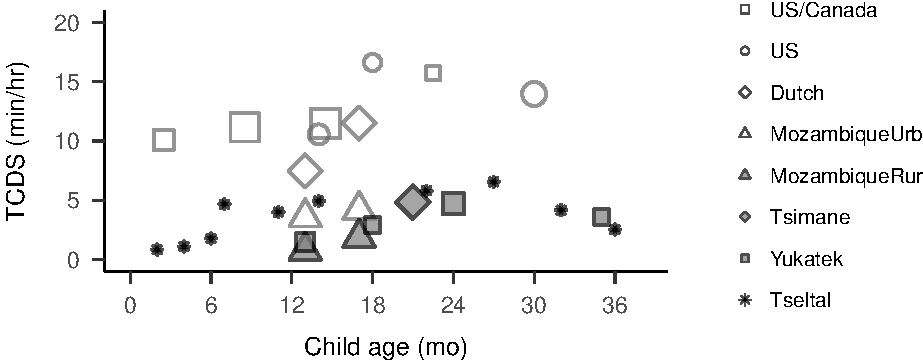
\includegraphics{Tseltal-CLE_files/figure-latex/fig4-1.pdf}
\caption{\label{fig:fig4}TCDS rate reported from daylong recordings made in
different populations, including both urban (gray) and rural/indigenous
(black) samples. Each point is the average TCDS rate reported for
children at the indicated age, and size indicates number of children
sampled (range: 1--26). See text for references to original studies.}
\end{figure}

The rate of TCDS in the randomly sampled clips was primarily affected by
factors relating to the time of day. The count model showed that,
overall, children were more likely to hear TCDS in the mornings and
evenings than around midday (B = 4.32, SD = 1.92, z = 2.25, p = 0.02).
However, this pattern weakened for older children, some of whom even
heard peak TCDS input around midday, as illustrated in
\protect\hyperlink{fig5}{Figure 5} (B = -5.22, SD = 1.97, z = -2.64, p =
0.01). There were no significant effects of child age, household size,
or number of speakers present, no significant effects in the
zero-inflation model.\footnote{This TCDS zero-inflation did not include
  the number of speakers present or time of day.}

\begin{figure}
\centering
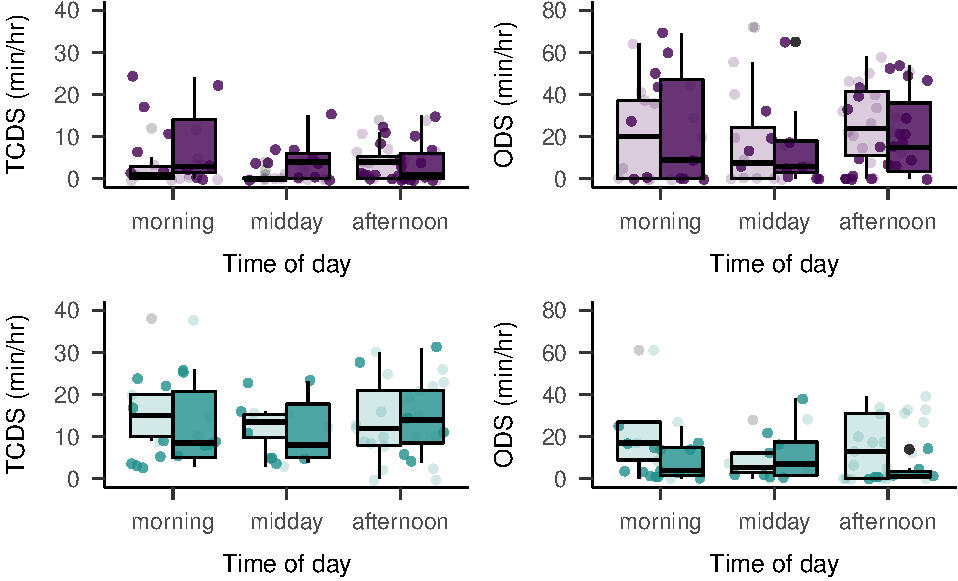
\includegraphics{Tseltal-CLE_files/figure-latex/fig5-1.pdf}
\caption{\label{fig:fig5}TCDS rate heard at different times of day by
children 12 months and younger (left) and 13 months and older (right) in
the randomly selected (purple) and turn-taking (green) clips.}
\end{figure}

In contrast to findings from Laura A Shneidman and Goldin-Meadow (2012)
on Yucatec Mayan, most TCDS in the current data came from adult speakers
(mean = 80.61\%, median = 87.22\%, range = 45.90\%--100), with no
evidence for an increase in proportion TCDS from children with target
child age (correlation between child age and proportion TCDS from
children: Spearman's \emph{rho} = -0.29; \emph{p} = 0.42).

\subsection{Other-directed speech
(ODS)}\label{other-directed-speech-ods}

Children heard an average of 21.05 minutes per hour in the random sample
(median = 17.80; range = 3.57--42.80): that is, 5--6 times as much
speech as was directed to them. We modeled ODS min/hr in the random
clips with a zero-inflated negative binomial regression, as described
above.

The count model of ODS in the randomly selected clips revealed that the
presence of more speakers was strongly associated with more ODS (B =
1.06, SD = 0.09, z = 11.54, p = 0). Additionally, more ODS occurred in
the mornings and evenings (B = 2.70, SD = 1.14, z = 2.36, p = 0.02), and
was also more frequent in large households for older children compared
to younger children (B = 0.33, SD = 0.16, z = 2.01, p = 0.04). There
were no other significant effects on ODS rate, and no significant
effects in the zero-inflation models.\footnote{This ODS count model did
  not include by-child intercepts of time of day and its zero-inflation
  did not include the number of speakers present.}

Other-directed speech may have been so common because there were an
average 3.44 speakers present other than the target child in the
randomly selected clips (median = 3; range = 0--10), and (typically)
more than half of the speakers were adults. However, these estimates may
be comparable to North American infants (6--7 months) living in nuclear
family homes (Bergelson et al., 2018a), so a high incidence of ODS may
be common for infants in many sociocultural contexts.

\begin{figure}
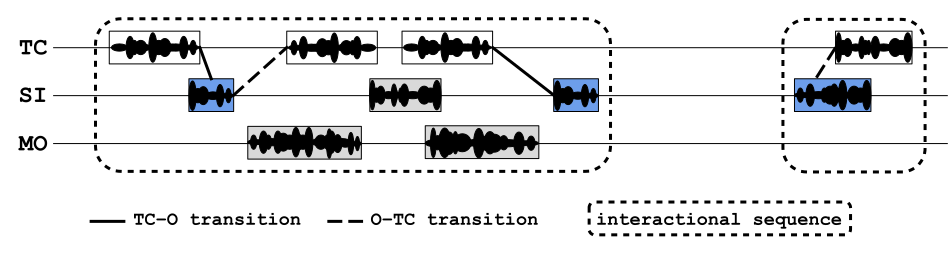
\includegraphics[width=1\linewidth]{Tseltal-CLE_files/TseltalCLE-TurnTimingIllustration} \caption{Illustration of a transcript clip between the target child (TCH), an older sister (SIS), and mother (MOT) in which transitions between the target child and other interlocutors are marked in solid and dashed lines and in which interactional sequences are marked with dotted lines. Light gray boxes indicate TCDS and dark gray boxes indicate ODS.}\label{fig:fig6}
\end{figure}

\subsection{Target-child-to-other turn transitions
(TC--O)}\label{target-child-to-other-turn-transitions-tco}

We detect contingent turn exchanges between the target child and other
speakers based on turn timing \protect\hyperlink{fig6}{Figure 6}. If a
child's vocalization is followed by a target-child-directed utterance
within -1000--2000msec of the end of the child's vocalization (Casillas,
Bobb, \& Clark, 2016; Hilbrink, Gattis, \& Levinson, 2015), it is
counted as a contingent response (i.e., a TC--O transition). We use the
same idea to find other-to-target-child transitions below (i.e., a
target-child-directed utterance followed by a target child vocalization
with the same overlap/gap restrictions). Each target child vocalization
can only have one prompt and one response and each target-child-directed
utterance can maximally count once as a prompt and once as a response
(e.g., in a TC--O--TC sequence, the \enquote{O} is both a response and a
prompt).

Gap and overlap restrictions are based on prior studies of infant and
young children's turn taking (Casillas et al., 2016; Hilbrink et al.,
2015), though the timing margins are increased slightly for the current
dataset because the prior estimates come from relatively short, intense
bouts of interaction in WEIRD parental contexts. Note, too, that much
prior work has used maximum gaps of similar or greater length to detect
verbal contingencies in caregiver-child interaction; and any work based
on LENA\^{}TM conversational blocks is thereby based on a 5-second
silence maximum (Bergelson et al., 2018b; M. H. Bornstein, Putnick,
Cote, Haynes, \& Suwalsky, 2015; Broesch, Rochat, Olah, Broesch, \&
Henrich, 2016; Egeren, Barratt, \& Roach, 2001; Y. Kuchirko, Tafuro, \&
Tamis-LeMonda, 2018; Romeo et al., 2018); in comparison our timing
restrictions are quite stringent.

\begin{figure}
\centering
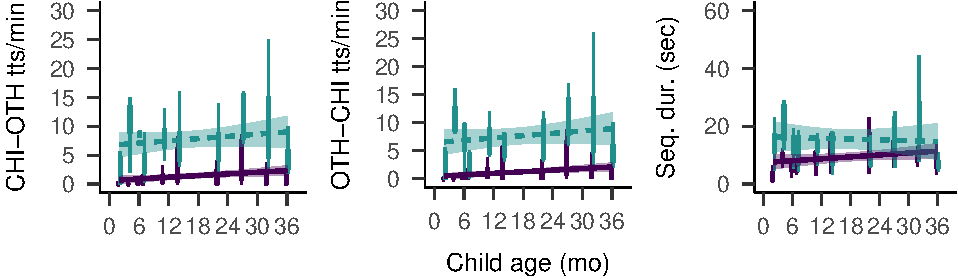
\includegraphics{Tseltal-CLE_files/figure-latex/fig7-1.pdf}
\caption{\label{fig:fig7}By-child estimates of contingent responses per
minute to the target child's vocalizations (left), contingent responses
per minute by the target child to others' target-child-directed speech
(middle), and the average duration of contingent interactional sequences
(right). Each datapoint represents the value for a single clip within
the random (purple; solid) or turn taking (green; dashed) samples. Bands
on the solid linear trends show 95\% CIs.}
\end{figure}

Other speakers responded contingently to the target children's
vocalizations at an average rate of 1.38 transitions per minute (median
= 0.40; range = 0--8.60). We modeled TC--O transtions per minute in the
random clips with a zero-inflated negative binomial regression, as
described above.

The rate at which children hear contingent response from others was
primarily influenced by factors relating to the child's age. Older
children heard more contingent responses then younger children when
there were more speakers present (B = 0.47, SD = 0.22, z = 2.11, p =
0.03). Also, as with the speech quantity measures, younger children
heard more contingent responses in the mornings and evenings while this
effect was less pronounced for older children (B = -6.46, SD = 2.56, z =
-2.52, p = 0.01).There were no other significant effects on TC--O
transition rate, and no significant effects in the zero-inflation model
either.\footnote{This TC--O transition count model did not include
  by-child intercepts of time of day.}

\subsection{Other-to-target-child turn transitions
(O--TC)}\label{other-to-target-child-turn-transitions-otc}

Tseltal children responded contingently to others' target-child
vocalizations at an average rate of 1.17 transitions per minute (median
= 0.20; range = 0--8.80). We modeled O--TC transtions per minute in the
random clips with a zero-inflated negative binomial regression, as
described above.

The rate at which children respond contingently to others (O--TC turn
transitions per minute) was similarly influenced by child age and time
of day: older children were less likely than young children to show peak
response rates in the morning and evening (B = -7.30, SD = 2.61, z =
-2.80, p = 0.01). There were no further significant effects in the count
or zero-inflation models.\footnote{This O--TC transition count model did
  not include by-child intercepts of time of day.}

\subsection{Sequence duration}\label{sequence-duration}

Sequences of interaction include periods of contingent turn taking with
at least one target child vocalization and one target-child-directed
prompt or response from another speaker. We use the same mechanism as
before to detect contingent TC--O and O--TC transitions, but also allow
for speakers to continue with multiple vocalizations in a row (e.g.,
TC--O--O--TC--OTH; \protect\hyperlink{fig7}{Figure 7}. Sequences are
bounded by the earliest and latest vocalization for which there is no
contingent prompt/response, respectively. Each target child vocalization
can only appear in one sequence, and many sequences have more than one
child vocalization. Because sequence durations were not zero-inflated,
we modeled them in the random clips with negative binomial regression.

We detected 311 interactional sequences in the 90 randomly selected
clips, with an average sequence duration of 10.13 seconds (median = 7;
range = 0.56--85.47). The average number of child vocalizations within
these sequences was 3.75 (range = 1--29; median = 3). None of the
predictors significantly impacted sequence duration (all \emph{p}
\textgreater{} 0.09).\footnote{This sequence duration model did not
  include by-child intercepts of time of day.}

\subsection{Peak interaction}\label{peak-interaction}

As expected, the turn-taking clips featured a much higher rate of
contingent turn transitions: the average TC--O transition rate was 7.73
transitions per minute (median = 7.80; range = 0--25) and the average
O--TC rate was 7.56 transitions per minute (median = 6.20; range =
0--26). The interactional sequences were also longer on average: 12.27
seconds (median = 8.10; range = 0.55--61.22).

Crucially, children also heard much more TCDS in the turn-taking
clips---13.28 min/hr (median = 13.65; range = 7.32--20.19)---while also
hearing less ODS---11.93 min/hr (median = 10.18; range = 1.37--24.42).

We modeled each of these five speech environment measures with parallel
models to those used above (with no zero-inflation model for TCDS,
TC--O, and O--TC rates, given the nature of the sample). The impact of
child age, time of day, household size, and number of speakers was
qualitatively similar (basic sample comparisons are visualized in
\protect\hyperlink{fig3}{Figure 3}, \protect\hyperlink{fig4}{Figure 4},
and \protect\hyperlink{fig6}{Figure 6}) between the randomly selected
clips and these peak periods of interaction with the following
exceptions: older children heard significantly less ODS (B = -0.49, SD =
NA, z = NA, p = NA), the presence of more speakers significantly
decreased children's response rate to other's vocalizations (B = -0.26,
SD = 0.12, z = -2.19, p = 0.03), and children's interactional sequences
were shorter for older children (B = -0.24, SD = 0.10, z = -2.42, p =
0.02), shorter for children in large households (B = -0.21, SD = 0.10, z
= -2.25, p = 0.02), and longer during peak periods in the mornings and
afternoons (B = 2.76, SD = 1.11, z = 2.50, p = 0.01). Full model outputs
can be compared in the Supplementary Materials.

\subsubsection{Peak minutes in the day}\label{peak-minutes-in-the-day}

We used these interactional characteristics to find similar
\enquote{high turn taking} minutes in the random samples in order to
extrapolate to the number of high interactivity minutes in the whole
day. To do this, we scanned each 60-second window (e.g., 0--60 sec,
1--61 sec, etc.\footnote{60 seconds is the smallest clip sample size in
  the turn-taking segments}) of each random clip from each child and
recorded the observed turn-transition rate. Only 6 of the 10 children
showed at least one minute of their random sample that equalled or
exceeded the grand average turn-transition rate (12.89 transitions per
minute), and 7 of the 10 children showed at least one minute equalling
or exceeding their own average turn transition rate from their
turn-taking samples, as shown in \protect\hyperlink{fig8}{Figure 8}.
Across children who did show turn-taking \enquote{peaks} in their random
data (i.e., at or above rates from the sample-average from the
turn-taking segments), periods of \enquote{peak} interaction were
relatively long, ranging in duration from an average of 0 to 103 seconds
across the 6 children with such peaks.

\begin{figure}
\centering
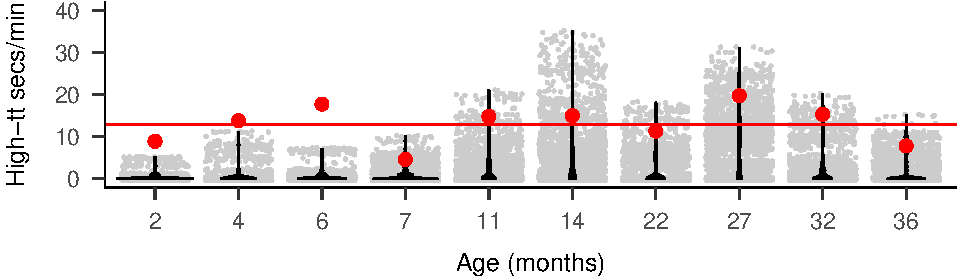
\includegraphics{Tseltal-CLE_files/figure-latex/fig8-1.pdf}
\caption{\label{fig:fig8}Turn-transitions rates, estimated over the last 60
seconds for each second of the random samples by child (nine 5-min clips
each). The horizontal line indicates the group mean turn-transition rate
in the turn-taking sample. The large points indicate the by-child mean
turn-transition rate in the turn-taking sample.}
\end{figure}

Assuming approximately 12 waking hours, we therefore very roughly
estimate that these Tseltal children spent an average of 100.16 minutes
(1.67 hours) in high turn-taking, dyadic interaction during their
recording day. However, the range in the quantity of high turn-taking
interaction varies enormously across children, starting at just a few
minutes per day and topping out at more than 419.73 minutes (7 hours) in
our sample.

\section{Discussion}\label{disc}

\subsection{Future directions}\label{disc-future}

\subsection{Conclusion}\label{disc-conclusion}

\section{Acknowledgements}\label{acknowledgements}

\newpage

\section{References}\label{refs}

\begingroup
\setlength{\parindent}{-0.5in} \setlength{\leftskip}{0.5in}

\hypertarget{refs}{}
\hypertarget{ref-abney2018bursts}{}
Abney, D. H., Dale, R., Louwerse, M. M., \& Kello, C. T. (2018). The
bursts and lulls of multimodal interaction: Temporal distributions of
behavior reveal differences between verbal and non-verbal communication.
\emph{Cognitive Science}, \emph{XX}, XX--XX.
doi:\href{https://doi.org/10.1111/cogs.12612}{10.1111/cogs.12612}

\hypertarget{ref-abney2017time}{}
Abney, D. H., Smith, L. B., \& Yu, C. (2017). It's time: Quantifying the
relevant time scales for joint attention. In G. Gunzelmann, A. Howes, T.
Tenbrink, \& E. Davelaar (Eds.), \emph{Proceedings of the 39th annual
meeting of the cognitive science society} (pp. 1489--1494). London, UK.

\hypertarget{ref-ambridge2006distributed}{}
Ambridge, B., Theakston, A. L., Lieven, E. V., \& Tomasello, M. (2006).
The distributed learning effect for children's acquisition of an
abstract syntactic construction. \emph{Cognitive Development},
\emph{21}(2), 174--193.

\hypertarget{ref-arnold2004avoiding}{}
Arnold, J. E., Wasow, T., Asudeh, A., \& Alrenga, P. (2004). Avoiding
attachment ambiguities: The role of constituent ordering. \emph{Journal
of Memory and Language}, \emph{51}(1), 55--70.

\hypertarget{ref-aslin1996models}{}
Aslin, R. N., Woodward, J. Z., LaMendola, N. P., \& Bever, T. G. (1996).
Models of word segmentation in fluent maternal speech to infants. In J.
L. Morgan \& K. Demuth (Eds.), \emph{Signal to syntax: Bootstrapping
from speech to grammar in early acquisition} (pp. 117--134). New York,
NY: Psychology Press.

\hypertarget{ref-barrett2013early}{}
Barrett, H., Broesch, T., Scott, R. M., He, Z., Baillargeon, R., Wu, D.,
\ldots{} Stephen Laurence. (2013). Early false-belief understanding in
traditional non-Western societies. \emph{Proceedings of the Royal
Society B: Biological Sciences}, \emph{280}(1755), XX--XX.
doi:\href{https://doi.org/10.1098/rspb.2012.2654}{10.1098/rspb.2012.2654}

\hypertarget{ref-bergelson2018day}{}
Bergelson, E., Amatuni, A., Dailey, S., Koorathota, S., \& Tor, S.
(2018a). Day by day, hour by hour: Naturalistic language input to
infants. \emph{Developmental Science}, \emph{XX}, XX--XX.

\hypertarget{ref-bergelsoncasillas2018what}{}
Bergelson, E., Casillas, M., Soderstrom, M., Seidl, A., Warlaumont, A.
S., \& Amatuni, A. (2018b). What do north american babies hear? A
large-scale cross-corpus analysis. \emph{Developmental Science},
\emph{XX}, XX--XX.

\hypertarget{ref-blasiIPhuman}{}
Blasi, D., Schikowski, R., Moran, S., Pfeiler, B., \& Stoll, S. (in
preparation). Human communication is structured efficiently for first
language learners: Lexical spikes.

\hypertarget{ref-bornstein2015mother}{}
Bornstein, M. H., Putnick, D. L., Cote, L. R., Haynes, O. M., \&
Suwalsky, J. T. D. (2015). Mother-infant contingent vocalizations in 11
countries. \emph{Psychological Science}, \emph{26}(8), 1272--1284.

\hypertarget{ref-brinchmann2019direct}{}
Brinchmann, E. I., Braeken, J., \& Lyster, S.-A. H. (2019). Is there a
direct relation between the development of vocabulary and grammar?
\emph{Developmental Science}, \emph{22}(1), e12709.

\hypertarget{ref-broesch2016similarities}{}
Broesch, T., Rochat, P., Olah, K., Broesch, J., \& Henrich, J. (2016).
Similarities and differences in maternal responsiveness in three
societies: Evidence from Fiji, Kenya, and the United States. \emph{Child
Development}, \emph{87}(3), 700--711.

\hypertarget{ref-R-glmmTMB}{}
Brooks, M. E., Kristensen, K., van Benthem, K. J., Magnusson, A., Berg,
C. W., Nielsen, A., \ldots{} Bolker, B. M. (2017a). glmmTMB balances
speed and flexibility among packages for zero-inflated generalized
linear mixed modeling. \emph{The R Journal}, \emph{9}(2), 378--400.
Retrieved from
\url{https://journal.r-project.org/archive/2017/RJ-2017-066/index.html}

\hypertarget{ref-brooks2017modeling}{}
Brooks, M. E., Kristensen, K., van Benthem, K. J., Magnusson, A., Berg,
C. W., Nielsen, A., \ldots{} Bolker, B. M. (2017b). Modeling
zero-inflated count data with glmmTMB. \emph{bioRxiv}.
doi:\href{https://doi.org/10.1101/132753}{10.1101/132753}

\hypertarget{ref-brown1998conversational}{}
Brown, P. (8AD). Conversational structure and language acquisition: The
role of repetition in tzeltal adult and child speech. \emph{Journal of
Linguistic Anthropology}, \emph{2}, 197--221.
doi:\href{https://doi.org/10.1525/jlin.1998.8.2.197}{10.1525/jlin.1998.8.2.197}

\hypertarget{ref-brown2011cultural}{}
Brown, P. (2011). The cultural organization of attention. In A. Duranti,
E. Ochs, \& and B.B. Schieffelin (Eds.), \emph{Handbook of language
socialization} (pp. 29--55). Malden, MA: Wiley-Blackwell.

\hypertarget{ref-brown2014interactional}{}
Brown, P. (2014). The interactional context of language learning in
tzeltal. In I. Arnon, M. Casillas, C. Kurumada, \& B. Estigarribia
(Eds.), \emph{Language in interaction: Studies in honor of eve v. clark}
(pp. 51--82). Amsterdam, NL: John Benjamins.

\hypertarget{ref-brownIPchildrearing}{}
Brown, P., \& Casillas, M. (in press). Childrearing through social
interaction on rossel island, png. In A. J. Fentiman \& M. Goody (Eds.),
\emph{Esther goody revisited: Exploring the legacy of an original
inter-disciplinarian} (pp. XX--XX). New York, NY: Berghahn.

\hypertarget{ref-brown2014language}{}
Brown, P., \& Gaskins, S. (2014). Language acquisition and language
socialization. In N. J. Enfield, P. Kockelman, \& J. Sidnell (Eds.),
\emph{Handbook of linguistic anthropology} (pp. 183--222). Cambridge,
UK: Cambridge University Press.

\hypertarget{ref-brown1997introduction}{}
Brown, R. (1977). Introduction. In C. E. Snow \& C. A. Ferguson (Eds.),
\emph{Talking to children: Language input and interaction} (pp. 1--30).
Cambridge, UK: Cambridge University Press.

\hypertarget{ref-bruner1985childs}{}
Bruner, J. (1985). \emph{Child's talk}. Oxford: Oxford University Press.

\hypertarget{ref-butterworth2003pointing}{}
Butterworth, G. (2003). Pointing is the royal road to language for
babies. In S. Kita (Ed.), \emph{Pointing} (pp. 17--42). Psychology
Press.

\hypertarget{ref-cartmill2013quality}{}
Cartmill, E. A., Armstrong, B. F., Gleitman, L. R., Goldin-Meadow, S.,
Medina, T. N., \& Trueswell, J. C. (2013). Quality of early parent input
predicts child vocabulary 3 years later. \emph{Proceedings of the
National Academy of Sciences}, \emph{110}(28), 11278--11283.

\hypertarget{ref-casillas2016turn}{}
Casillas, M., Bobb, S. C., \& Clark, E. V. (2016). Turn taking, timing,
and planning in early language acquisition. \emph{Journal of Child
Language}, \emph{43}, 1310--1337.

\hypertarget{ref-Casillas-HB}{}
Casillas, M., Brown, P., \& Levinson, S. C. (2017). Casillas HomeBank
corpus.

\hypertarget{ref-casillas2017ACLEWDAS}{}
Casillas, M., Bunce, J., Soderstrom, M., Rosemberg, C., Migdalek, M.,
Alam, F., \ldots{} Garrison, H. (2017). Introduction: The aclew das
template {[}training materials{]}. Retrieved from
\url{https://osf.io/aknjv/}

\hypertarget{ref-childers2002two}{}
Childers, J. B., \& Tomasello, M. (2002). Two-year-olds learn novel
nouns, verbs, and conventional actions from massed or distributed
exposures. \emph{Developmental Psychology}, \emph{38}(6), 967--978.
doi:\href{https://doi.org/10.1037//0012-1649.38.6.967}{10.1037//0012-1649.38.6.967}

\hypertarget{ref-chouinard2003adult}{}
Chouinard, M. M., \& Clark, E. V. (2003). Adult reformulations of child
errors as negative evidence. \emph{Journal of Child Language},
\emph{30}(3), 637--669.

\hypertarget{ref-cooper1990preference}{}
Cooper, R. P., \& Aslin, R. N. (1990). Preference for infant-directed
speech in the first month after birth. \emph{Child Development},
\emph{20}(4), 477--488.
doi:\href{https://doi.org/10.1016/S0163-6383(97)90037-0}{10.1016/S0163-6383(97)90037-0}

\hypertarget{ref-cristia2013input}{}
Cristia, A. (2013). Input to language: The phonetics and perception of
infant-directed speech. \emph{Language and Linguistics Compass},
\emph{7}(3), 157--170.
doi:\href{https://doi.org/10.1111/lnc3.12015}{10.1111/lnc3.12015}

\hypertarget{ref-cristia2017child}{}
Cristia, A., Dupoux, E., Gurven, M., \& Stieglitz, J. (2017).
Child-directed speech is infrequent in a forager-farmer population: A
time allocation study. \emph{Child Development}, XX--XX.
doi:\href{https://doi.org/10.1111/cdev.12974}{10.1111/cdev.12974}

\hypertarget{ref-demuth2010three}{}
Demuth, K., Moloi, F., \& Machobane, M. (2010). 3-year-olds'
comprehension, production, and generalization of Sesotho passives.
\emph{Cognition}, \emph{115}(2), 238--251.

\hypertarget{ref-vanegeren2001mother}{}
Egeren, L. A. van, Barratt, M. S., \& Roach, M. A. (2001). Mother-infant
responsiveness: Timing, mutual regulation, and interactional context.
\emph{Developmental Psychology}, \emph{37}(5), 684--697.

\hypertarget{ref-estigarribia2007getting}{}
Estigarribia, B., \& Clark, E. V. (2007). Getting and maintaining
attention in talk to young children. \emph{Journal of Child Language},
\emph{34}(4), 799--814.

\hypertarget{ref-fortierURadhoc}{}
Fortier, M. E., Kellier, D., Fernández Flecha, M., \& Frank, M. C.
(under review). Ad-hoc pragmatic implicatures among Shipibo-Konibo
children in the Peruvian Amazon.
doi:\href{https://doi.org/10.31234/osf.io/x7ad9}{10.31234/osf.io/x7ad9}

\hypertarget{ref-frankIPvariability}{}
Frank, M. C., Braginsky, M., Marchman, V., \& Yurovsky, D. (n.d.).
\emph{Variability and consistency in early language learning: The
Wordbank project}. XX. Retrieved from
\url{https://langcog.github.io/wordbank-book/}

\hypertarget{ref-fusaroli2014synergy}{}
Fusaroli, R., Razczaszek-Leonardi, J., \& Tylén, K. (2014). Dialog as
interpersonal synergy. \emph{New Ideas in Psychology}, \emph{32},
147--157.
doi:\href{https://doi.org/10.1016/j.newideapsych.2013.03.005}{10.1016/j.newideapsych.2013.03.005}

\hypertarget{ref-ganek2018using}{}
Ganek, H., Smyth, R., Nixon, S., \& Eriks-Brophy, A. (2018). Using the
Language ENvironment analysis (LENA) system to investigate cultural
differences in conversational turn count. \emph{Journal of Speech,
Language, and Hearing Research}, \emph{61}, 2246--2258.
doi:\href{https://doi.org/10.1044/2018_JSLHR-L-17-0370}{10.1044/2018\_JSLHR-L-17-0370}

\hypertarget{ref-garcia2018thematic}{}
Garcia, R., Roeser, J., \& Höhle, B. (2018). Thematic role assignment in
the L1 acquisition of Tagalog: Use of word order and morphosyntactic
markers. \emph{Language Acquisition}, \emph{XX}, XX--XX.
doi:\href{https://doi.org/10.1080/10489223.2018.1525613}{10.1080/10489223.2018.1525613}

\hypertarget{ref-gaskins1996how}{}
Gaskins, S. (1996). How Mayan parental theories come into play.
\emph{Parents' Cultural Belief Systems: Their Origins, Expressions, and
Consequences}, 345--363.

\hypertarget{ref-gaskins1999childrens}{}
Gaskins, S. (1999). Children's daily lives in a Mayan village: A case
study of culturally constructed roles and activities. In A. Göncü (Ed.),
\emph{Children's engagement in the world: Sociocultural perspectives}
(pp. 25--60). Oxford: Berg.

\hypertarget{ref-gaskins2006cultural}{}
Gaskins, S. (2006). Cultural perspectives on infant--caregiver
interaction. In N. J. Enfield \& S. Levinson (Eds.), \emph{Roots of
human sociality: Culture, cognition and interaction} (pp. 279--298).
Oxford: Berg.

\hypertarget{ref-goldberg2003constructions}{}
Goldberg, A. E. (2003). Constructions: A new theoretical approach to
language. \emph{Trends in Cognitive Sciences}, \emph{7}(5), 219--224.

\hypertarget{ref-golinkoff2015baby}{}
Golinkoff, R. M., Can, D. D., Soderstrom, M., \& Hirsh-Pasek, K. (2015).
(Baby) talk to me: The social context of infant-directed speech and its
effects on early language acquisition. \emph{Current Directions in
Psychological Science}, \emph{24}(5), 339--344.

\hypertarget{ref-greenwood2011assessing}{}
Greenwood, C. R., Thiemann-Bourque, K., Walker, D., Buzhardt, J., \&
Gilkerson, J. (2011). Assessing children's home language environments
using automatic speech recognition technology. \emph{Communication
Disorders Quarterly}, \emph{32}(2), 83--92.
doi:\href{https://doi.org/10.1177/1525740110367826}{10.1177/1525740110367826}

\hypertarget{ref-hart1995meaningful}{}
Hart, B., \& Risley, T. R. (1995). \emph{Meaningful Differences in the
Everyday Experience of Young American Children}. Paul H. Brookes
Publishing.

\hypertarget{ref-henrich2010beyond}{}
Henrich, J., Heine, S. J., \& Norenzayan, A. (2010). Beyond WEIRD:
Towards a broad-based behavioral science. \emph{Behavioral and Brain
Sciences}, \emph{33}(2--3), 111--135.

\hypertarget{ref-hernik2018infant}{}
Hernik, M., \& Broesch, T. (2018). Infant gaze following depends on
communicative signals: An eye-tracking study of 5- to 7-month-olds in
Vanuatu. \emph{Developmental Science}, \emph{XX}, XX--XX.
doi:\href{https://doi.org/10.1111/desc.12779}{10.1111/desc.12779}

\hypertarget{ref-hilbrink2015early}{}
Hilbrink, E., Gattis, M., \& Levinson, S. C. (2015). Early developmental
changes in the timing of turn-taking: A longitudinal study of
mother--infant interaction. \emph{Frontiers in Psychology},
\emph{6:1492}, 1--12.

\hypertarget{ref-hirshpasek2015contribution}{}
Hirsh-Pasek, K., Adamson, L. B., Bakeman, R., Owen, M. T., Golinkoff, R.
M., Pace, A., \ldots{} Suma, K. (2015). The contribution of early
communication quality to low-income children's language success.
\emph{Psychological Science}, \emph{26}(7), 1071--1083.
doi:\href{https://doi.org/10.1177/0956797615581493}{10.1177/0956797615581493}

\hypertarget{ref-hoff2003specificity}{}
Hoff, E. (2003). The specificity of environmental influence:
Socioeconomic status affects early vocabulary development via maternal
speech. \emph{Child Development}, \emph{74}(5), 1368--1378.

\hypertarget{ref-hoff2006social}{}
Hoff, E. (2006). How social contexts support and shape language
development. \emph{Developmental Review}, \emph{26}(1), 55--88.

\hypertarget{ref-hurtado2008does}{}
Hurtado, N., Marchman, V. A., \& Fernald, A. (2008). Does input
influence uptake? Links between maternal talk, processing speed and
vocabulary size in spanish-learning children. \emph{Developmental
Science}, \emph{11}(6), F31--F39.
doi:\href{https://doi.org/10.1111/j.1467-7687.2008.00768.x\%5D}{10.1111/j.1467-7687.2008.00768.x{]}}

\hypertarget{ref-huttenlocher2010sources}{}
Huttenlocher, J., Waterfall, H., Vasilyeva, M., Vevea, J., \& Hedges, L.
V. (2010). Sources of variability in children's language growth.
\emph{Cognitive Psychology}, \emph{61}, 343--365.

\hypertarget{ref-kuchirko2017becoming}{}
Kuchirko, Y., Tafuro, L., \& Tamis-LeMonda, C. S. (2018). Becoming a
communicative partner: Infant contingent responsiveness to maternal
language and gestures. \emph{Infancy}, \emph{23}(4), 558--576.

\hypertarget{ref-deleon1998emergent}{}
León, L. de. (1998). The emergent participant: Interactive patterns in
the socialization of Tzotzil (Mayan) infants. \emph{Journal of
Linguistic Anthropology}, \emph{8}(2), 131--161.

\hypertarget{ref-deleon2011language}{}
León, L. de. (2011). Language socialization and multiparty participation
frameworks. In A. Duranti, E. Ochs, \& and B.B. Schieffelin (Eds.),
\emph{Handbook of language socialization} (pp. 81--111). Malden, MA:
Wiley-Blackwell.
doi:\href{https://doi.org/10.1002/9781444342901.ch4}{10.1002/9781444342901.ch4}

\hypertarget{ref-lieven1994crosslinguistic}{}
Lieven, E. V. M. (1994). Crosslinguistic and crosscultural aspects of
language addressed to children. In C. Gallaway \& B. J. Richards (Eds.),
\emph{Input and interaction in language acquisition} (pp. 56--73). New
York, NY, US: Cambridge University Press.
doi:\href{https://doi.org/10.1017/CBO9780511620690.005}{10.1017/CBO9780511620690.005}

\hypertarget{ref-lieven1997lexically}{}
Lieven, E. V. M., Pine, J. M., \& Baldwin, G. (1997). Lexically-based
learning and early grammatical development. \emph{Journal of Child
Language}, \emph{24}(1), 187--219.

\hypertarget{ref-liszkowski2012prelinguistic}{}
Liszkowski, U., Brown, P., Callaghan, T., Takada, A., \& De Vos, C.
(2012). A prelinguistic gestural universal of human communication.
\emph{Cognitive Science}, \emph{36}(4), 698--713.

\hypertarget{ref-marchman2004language}{}
Marchman, V. A., Martínez-Sussmann, C., \& Dale, P. S. (2004). The
language-specific nature of grammatical development: Evidence from
bilingual language learners. \emph{Developmental Science}, \emph{7}(2),
212--224.

\hypertarget{ref-masataka2003onset}{}
Masataka, N. (2003). \emph{The onset of language}. Cambridge University
Press.

\hypertarget{ref-mastin2016infant}{}
Mastin, J. D., \& Vogt, P. (2016). Infant engagement and early
vocabulary development: A naturalistic observation study of Mozambican
infants from 1;1 to 2;1. \emph{Journal of Child Language}, \emph{43}(2),
235--264.
doi:\href{https://doi.org/0.1017/S0305000915000148}{0.1017/S0305000915000148}

\hypertarget{ref-newport1977mother}{}
Newport, E. L., Gleitman, H., \& Gleitman, L. R. (1977). Mother, i'd
rather do it myself: Some effects and non-effects of maternal speech
style. In C. E. Snow \& C. A. Ferguson (Eds.), \emph{Talking to
children: Language input and interaction} (pp. 109--150). Cambridge, UK:
Cambridge University Press.

\hypertarget{ref-nielsen2017persistent}{}
Nielsen, M., Haun, D., Kärtner, J., \& Legare, C. H. (2017). The
persistent sampling bias in developmental psychology: A call to action.
\emph{Journal of Experimental Child Psychology}, \emph{162}, 31--38.

\hypertarget{ref-manybabies2017}{}
preference, Q. sources of variability in infancy research using the
infant-directed speech. (2017). ManyBabies collaborative. \emph{Advances
in Methods and Practices in Psychological Science}, \emph{XX}, XX--XX.
doi:\href{https://doi.org/10.31234/osf.io/s98ab}{10.31234/osf.io/s98ab}

\hypertarget{ref-pye1986quiche}{}
Pye, C. (1986). Quiché Mayan speech to children. \emph{Journal of Child
Language}, \emph{13}(1), 85--100.

\hypertarget{ref-pye2017comparative}{}
Pye, C. (2017). \emph{The comparative method of language acquisition
research}. University of Chicago Press.

\hypertarget{ref-R-base}{}
R Core Team. (2018). \emph{R: A language and environment for statistical
computing}. Vienna, Austria: R Foundation for Statistical Computing.
Retrieved from \url{https://www.R-project.org/}

\hypertarget{ref-ramirezesparza2014look}{}
Ramírez-Esparza, N., García-Sierra, A., \& Kuhl, P. K. (2014). Look
who's talking: Speech style and social context in language input to
infants are linked to concurrent and future speech development.
\emph{Developmental Science}, \emph{17}, 880--891.

\hypertarget{ref-ramirezesparza2017look}{}
Ramírez-Esparza, N., García-Sierra, A., \& Kuhl, P. K. (2017). Look
who's talking NOW! Parentese speech, social context, and language
development across time. \emph{Frontiers in Psychology}, \emph{8}, 1008.

\hypertarget{ref-rogoff1993guided}{}
Rogoff, B., Mistry, J., Göncü, A., Mosier, C., Chavajay, P., \& Heath,
S. B. (1993). Guided participation in cultural activity by toddlers and
caregivers. \emph{Monographs of the Society for Research in Child
Development}.

\hypertarget{ref-rogoff2003firsthand}{}
Rogoff, B., Paradise, R., Arauz, R. M., Correa-Chávez, M., \& Angelillo,
C. (2003). Firsthand learning through intent participation. \emph{Annual
Review of Psychology}, \emph{54}(1), 175--203.
doi:\href{https://doi.org/10.1146/annurev.psych.54.101601.145118}{10.1146/annurev.psych.54.101601.145118}

\hypertarget{ref-romeo2018beyond}{}
Romeo, R. R., Leonard, J. A., Robinson, S. T., West, M. R., Mackey, A.
P., Rowe, M. L., \& Gabrieli, J. D. (2018). Beyond the 30-million-word
gap: Children's conversational exposure is associated with
language-related brain function. \emph{Psychological Science},
\emph{29}(5), 700--710.

\hypertarget{ref-rowe2008child}{}
Rowe, M. L. (2008). Child-directed speech: Relation to socioeconomic
status, knowledge of child development and child vocabulary skill.
\emph{Journal of Child Language}, \emph{35}(1), 185--205.

\hypertarget{ref-salomo2013sociocultural}{}
Salomo, D., \& Liszkowski, U. (2013). Sociocultural settings influence
the emergence of prelinguistic deictic gestures. \emph{Child
Development}, \emph{84}(4), 1296--1307.

\hypertarget{ref-scaffIPlanguage}{}
Scaff, C., Stieglitz, J., Casillas, M., \& Cristia, A. (In preparation).
Language input in a hunter-forager population: Estimations from daylong
recordings.

\hypertarget{ref-schwab2016repetition}{}
Schwab, J. F., \& Lew-Williams, C. (2016). Repetition across successive
sentences facilitates young children's word learning.
\emph{Developmental Psychology}, \emph{52}(6), 879--886.

\hypertarget{ref-segal2015infant}{}
Segal, J., \& Newman, R. S. (2015). Infant preferences for structural
and prosodic properties of infant-directed speech in the second year of
life. \emph{Infancy}, \emph{20}(3), 339--351.
doi:\href{https://doi.org/10.1111/infa.12077}{10.1111/infa.12077}

\hypertarget{ref-shneidman2010language}{}
Shneidman, L. A. (2010). \emph{Language input and acquisition in a Mayan
village} (PhD thesis). The University of Chicago.

\hypertarget{ref-shneidman2012language}{}
Shneidman, L. A., \& Goldin-Meadow, S. (2012). Language input and
acquisition in a Mayan village: How important is directed speech?
\emph{Developmental Science}, \emph{15}(5), 659--673.

\hypertarget{ref-shneidman2012counts}{}
Shneidman, L. A., Arroyo, M. E., Levine, S. C., \& Goldin-Meadow, S.
(2012). What counts as effective input for word learning? \emph{Journal
of Child Language}, \emph{40}(3), 672--686.

\hypertarget{ref-smithson2013generalized}{}
Smithson, M., \& Merkle, E. (2013). \emph{Generalized linear models for
categorical and continuous limited dependent variables}. CRC Press: Boca
Raton.

\hypertarget{ref-soderstrom2007beyond}{}
Soderstrom, M. (2007). Beyond babytalk: Re-evaluating the nature and
content of speech input to preverbal infants. \emph{Developmental
Review}, \emph{27}(4), 501--532.

\hypertarget{ref-tamislemonda2017power}{}
Tamis-LeMonda, C., Kuchirko, Y., Luo, R., Escobar, K., \& Bornstein, M.
(2017). Power in methods: Language to infants in structured and
naturalistic contexts. \emph{Developmental Science}, \emph{20}(6),
XX--XX.
doi:\href{https://doi.org/doi.org/10.1111/desc.12456}{doi.org/10.1111/desc.12456}

\hypertarget{ref-HomeBank}{}
VanDam, M., Warlaumont, A. S., Bergelson, E., Cristia, A., De Palma, P.,
\& MacWhinney, B. (2016). HomeBank: An online repository of daylong
child-centered audio recordings. \emph{Seminars in Speech and Language}.

\hypertarget{ref-vogt2015communicative}{}
Vogt, P., Mastin, J. D., \& Schots, D. M. A. (2015). Communicative
intentions of child-directed speech in three different learning
environments: Observations from the netherlands, and rural and urban
mozambique. \emph{First Language}, \emph{35}(4-5), 341--358.

\hypertarget{ref-wasow1997remarks}{}
Wasow, T. (1997). Remarks on grammatical weight. \emph{Language
Variation and Change}, \emph{9}(1), 81--105.

\hypertarget{ref-weisleder2013talking}{}
Weisleder, A., \& Fernald, A. (2013). Talking to children matters: Early
language experience strengthens processing and builds vocabulary.
\emph{Psychological Science}, \emph{24}(11), 2143--2152.

\hypertarget{ref-R-ggplot2}{}
Wickham, H. (2009). \emph{Ggplot2: Elegant graphics for data analysis}.
Springer-Verlag New York. Retrieved from \url{http://ggplot2.org}

\hypertarget{ref-ELAN}{}
Wittenburg, P., Brugman, H., Russel, A., Klassmann, A., \& Sloetjes, H.
(2006). Elan: A professional framework for multimodality research. In
\emph{Proceedings of the fifth international conference on language
resources and evaluation}.

\hypertarget{ref-lucidIP}{}
XX. (XX). XX. \emph{XX}, \emph{XX}(XX), XX--XX.
doi:\href{https://doi.org/XX}{XX}

\endgroup






\end{document}
